\documentclass[12pt]{article}
\usepackage[a4paper,margin=.5in]{geometry}
\usepackage{graphicx}
\usepackage{booktabs}
\usepackage{listings}
\usepackage{color}

\definecolor{dkgreen}{rgb}{0,0.6,0}
\definecolor{gray}{rgb}{0.5,0.5,0.5}
\definecolor{mauve}{rgb}{0.58,0,0.82}

\lstset{frame=tb,
  language=Python,
  aboveskip=3mm,
  belowskip=3mm,
  showstringspaces=false,
  columns=flexible,
  basicstyle={\small\ttfamily},
  numbers=none,
  numberstyle=\tiny\color{gray},
  keywordstyle=\color{blue},
  commentstyle=\color{dkgreen},
  stringstyle=\color{mauve},
  breaklines=true,
  breakatwhitespace=true,
  tabsize=3
}
%\usepackage{subfig}
\usepackage{subcaption}
\usepackage{hyperref}
\hypersetup{
    colorlinks=true,
    linkcolor=blue,
    filecolor=magenta,      
    urlcolor=cyan,
    pdftitle={Overleaf Example},
    pdfpagemode=FullScreen,
    }
\newcommand*{\figuretitle}[1]{%
    {\centering%   <--------  will only affect the title because of the grouping (by the
    \textbf{#1}%              braces before \centering and behind \medskip). If you remove
    \par\medskip}%            these braces the whole body of a {figure} env will be centered.
}
\title{Homework 1 Writeup}

\author{Tylman Michael\\CSE 546 Machine Learning}
\date{1/22/2023}
%moderncv theme
\usepackage[utf8]{inputenc} 
\begin{document}
\maketitle{}
\section{KNN}

Starting off with the KNN, I abused the simplicity of the process and the power of my desktop to run the KNN algorithm
with neighbors ranging from 1 to 100. You can see the resulting $R^2$ value in Figure 1 for each neighbor chosen.

We can see that our training data starts off with perfect performance when we have 1 neighbor, which is as expected.
At this point, our model is wholly overfit. 
Normally I wouldn't point out this behavior, but it serves as an important sanity check for some of the results we 
will see later. 

Looking at the plot, we can see that our test and train curves actually meet and pass one another at about 35 neighbors.
This is very interesting behavior, which at first concerned me, but then I saw the pattern continue in the other models.

Regardless, we see our test performance quickly approach a peak and then begin to level out before 10 neighbors. 
Between 15 and 20 we see very little difference, and the very best test accuracy is occuring at neighbors=17. Past this 
point we begin to see diminishing returns where the model underfits too much. 
\begin{figure}
    \includegraphics[width=.95\textwidth]{../output/knn/plot.png}
    \caption{KNN Performance Graph}
    \label{image1}
\end{figure}

\section{OLS Regression}
For the OLS Regression, we see an $R^2$ score of 0.337 for the test data, and shockingly we see a value of 0.276 for the 
train data. I checked the cumulative percentage sum of eigenvalues to see how much information persists in the first 
dimension, which we can see in image 2.

Oddly, this data actually does appear to be able to be reduced down to a single dimension quite well. 98.8\% of the information
is held in the first eigenvector. Once I discovered this, I went to search for others who have worked on this dataset and I found
this \href{https://towardsdatascience.com/red-wine-quality-prediction-using-regression-modeling-and-machine-learning-7a3e2c3e1f46}{LINK}
which showed that they managed an $R^2$ score of .348 with some intentional feature selection.

So, I decided to redo my OLS regression after projecting my data into a lower dimension, and it actually got worse.
We went from an $R^2$ score of .337 to a score of .02. I think this is pretty strong evidence that the relationship 
between the information given to learn from, and the desired conclusion is nonlinear. Because while the information 
given to learn from can be reduced fairly well to be linear, the conclusion gained is not, as can be seen by the 
following 2D plot where I take the projection along the strongest dimension as the X-axis, and the quality as the Y-axis.

As we can see, although the first dimension contains 98.8 of the variance, there is no good relationship between this and 
the results of the quality test. As such, I cannot say that the linear method is a good fit.

As for the oddity that our testing performance was greater than our training performance, I think that is a behavior that stems 
from how poorly we are performing. I used the same functions for generating the plots and analysis for all models, and the behavior 
seen by our KNN can only be accomplished by performing the analysis correctly. At an $R^2$ of 0, we are equivalent to 
guessing just the mean of a random variable. Since we have such a weak performance, it doesn't surprise me that the smaller
set of the test data has less outliers and more easily correlates to our projected guesses.

\begin{figure}
  \begin{subfigure}{.5\textwidth}
  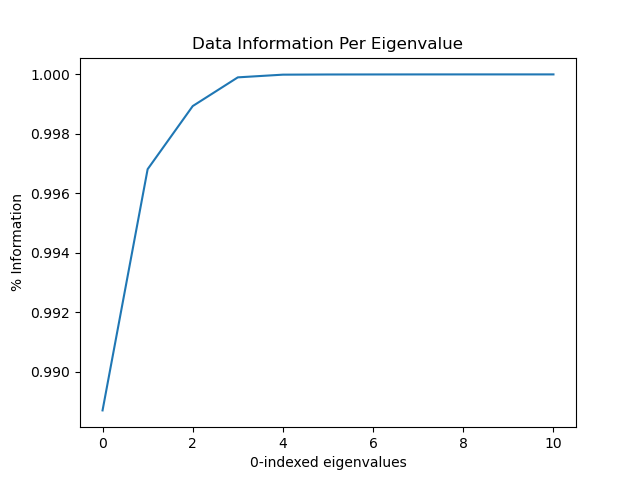
\includegraphics[width=.95\textwidth]{../Information.png}
  \caption{Information Distribution}
  \end{subfigure}%
  \begin{subfigure}{.5\textwidth}
  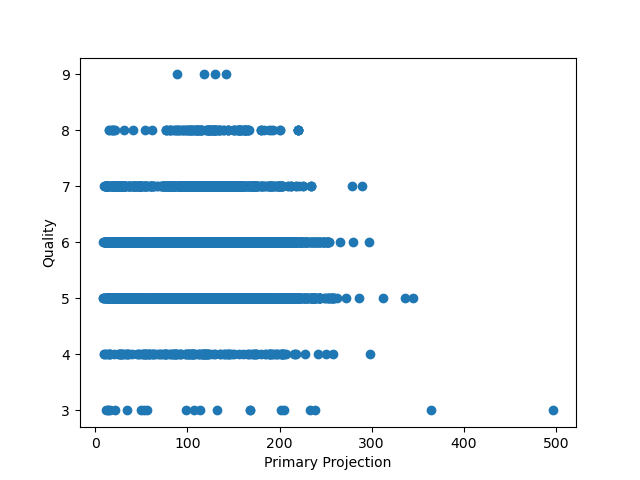
\includegraphics[width=.95\textwidth]{../SVD_Plot.png}
  \caption{SVD Plot}
  \end{subfigure}
\end{figure}

\section{Ridge Regression}
Moving on from the OLS, we employ Ridge Regression. This regularization is meant to limit the complexity of out model. 
As I stated before, our model isn't complex enough as it is. So we can expect any regularization to actually decrease 
efficacy. In this case, it's my hypothesis that the best value of alpha will be 0.

Looking at the plot and my results, we can see that this idea holds up as well. Our very best result is when alpha was
0, which is equivalent to the OLS case. As such, all of the performance has been analyzed already in the previous section.

\begin{figure}
  \includegraphics[width=.95\textwidth]{../output/ridge/plot.png}
  \caption{Ridge Performance Graph}
\end{figure}



\section{Lasso Regression}
Lasso Regression employs a regularization parameter like the Ridge regressor, so we might be tempted to follow the same logic.
Unfortunately, Lasso Regression actually has some additional functionality as it can drop the weight for features to 0.
This benefits us as it can perform some of it's own feature selection, which as we saw in the linked article can improve 
performance. 

The behavior here is a bit more complex, as there appear to be 3 distinct regions of behavior. First region is a stark, consistent
decrease in performance, the second region is a slower decline in performance along a curve, and the last is a steady decrease in performance.
I think the first region is where we can see the complexity limiting behavior of regularization dominate, in which our model 
loses performance since it was already lacking in complexity. The second region is where the feature selection behavior 
begins to be comparible to the complexity reduction, which leads to a slower decline. The final region is where the Alpha 
parameter begins to dominate the function as a whole, and we approach our asymptotic approach towards guessing only the mean.

Once again, we see the best result occuring at alpha = 0. As such, the analysis of performance coincides with OLS like the 
ridge regression did. In short, my justification for my choices of alpha = 0 for Ridge and Lasso Regression is connected to 
my belief that the OLS method already is underfit for the problem, and any attempt to limit its complexity will only 
exacerbate the issue.

\begin{figure}
  \includegraphics[width=.95\textwidth]{../output/lasso/plot.png}
  \caption{Lasso Performance Graph}
\end{figure}



\end{document}